\documentclass[Main.tex]{subfiles}
\begin{document}
	
	

\section{Intervals}

	\citet{BA99} note the similarity of limits of agreement to
	confidence intervals, but are clear that they are not the same
	thing. Interestingly, they describe the limits as ``being like a
	reference interval."
	
	Limits of agreement have very similar construction to Shewhart
	control limits. The Shewhart chart is a well known graphical
	methodology used in statistical process control. Consequently
	there is potential for misinterpreting the limits of agreement as
	if equivalent to Shewhart control limits. Importantly the
	parameters used to determine the limits, the mean and standard
	deviation, are not based on any sample used for an analysis, but
	on the process's historical values, a key difference with
	Bland-Altman limits of agreement.
	
	\citet{BXC2008} regards the limits of agreement as a prediction
	interval for the difference between future measurements with the
	two methods on a new individual, but states that it does not fit
	the formal definition of a prediction interval, since the
	definition does not consider the errors in estimation of the
	parameters. Prediction intervals, which are often used in
	regression analysis, are estimates of an interval in which future
	observations will fall, with a certain probability, given what has
	already been observed. \citet{BXC2008} offers an alternative
	formulation, a $95\%$ prediction interval for the difference
	\begin{equation}
	\bar{d} \pm t_{(0.975, n-1)}S_{d} \sqrt{1+\frac{1}{n}}
	\end{equation}
	
	\noindent where $n$ is the number of subjects. Only for 61 or more
	subjects is there a quantile less than 2.
	
	\citet{luiz} describes limits of agreement as tolerance limits. A
	tolerance interval for a measured quantity is the interval in
	which a specified fraction of the population's values lie, with a
	specified level of confidence.
	
	%At least 100 historical
	%values must be used to determine the acceptable value (i.e the
	%process mean) and the process standard deviation. The principle
	%that the mean and variance of a large sample of a homogeneous
	%population is a close approximation of the population's mean and
	%variance justifies this.
	
	


	
	\subsection{Purpose of Limits of Agreement} It must be established
	clearly the specific purpose of the limits of agreement.
	\citet*{BA95} comment that the limits of agreement \emph{how far
		apart measurements by the two methods were likely to be for most
		individuals.}, a definition echoed in their 1999 paper:
	\begin{quote} We can then say that nearly all pairs
		of measurements by the two methods will be closer together than
		these extreme values, which we call 95\% limits of agreement.
		These values define the range within which most differences
		between measurements by the two methods will lie\citep{BA99}.
	\end{quote}
	\citet{BXC} offers an alternative, more specific,  definition of
	the limits of agreement \emph{"a prediction interval for the
		difference between future measurements with the two methods on a
		new individual."} \citet{luiz} describes them as tolerance limits.
	
	Importantly they have the same construction as Shewhart Control
	limits.

\subsection{Formal definition of limits of agreement}
\citet{BA99} note the similarity of limits of agreement to
confidence intervals, but are clear that they are not the same
thing. Interestingly, they describe the limits as `being like a
reference interval'.

Limits of agreement have very similar construction to Shewhart
control limits. The Shewhart chart is a well known graphical
methodology used in statistical process control. Consequently
there is potential for misinterpreting the limits of agreement as
they were Shewhart control limits. 
%Importantly the
%parameters used to determine the Shewhart limits are time ordered, based on the process's historical values, a key difference with Bland-Altman limits of agreement.

\citet{BXC2008} regards the limits of agreement as a prediction
interval for the difference between future measurements with the
two methods on a new individual, but states that it does not fit
the formal definition of a prediction interval, since the
definition does not consider the errors in estimation of the
parameters. Prediction intervals, which are often used in
regression analysis, are estimates of an interval in which future
observations will fall, with a certain probability, given what has
already been observed. \citet{BXC2008} offers an alternative
formulation, a $95\%$ prediction interval for the difference
\[
\bar{d} \pm t_{(0.025, n-1)}s_{d} \sqrt{1+\frac{1}{n}}
\]

\noindent where $n$ is the number of subjects. Carstensen is
careful to consider the effect of the sample size on the interval
width, adding that only for 61 or more subjects is the
quantile less than 2.

\citet{luiz} offers an alternative description of limits of
agreement, this time as tolerance limits. A tolerance interval for
a measured quantity is the interval in which a specified fraction
of the population's values lie, with a specified level of
confidence. \citet{Barnhart} describes them as a probability
interval, and offers a clear description of how they should be
used; `if the absolute limit is less than an acceptable difference
$d_{0}$, then the agreement between the two methods is deemed
satisfactory'.

The prevalence of contradictory definitions of what limits of agreement strictly are will inevitably attenuate the poor standard of reporting using limits of agreement, as mentioned by \citet{mantha}.

%At least 100 historical
%values must be used to determine the acceptable value (i.e the
%process mean) and the process standard deviation. The principle
%that the mean and variance of a large sample of a homogeneous
%population is a close approximation of the population's mean and
%variance justifies this.

%\begin{figure}[h!]
%\begin{center}
%  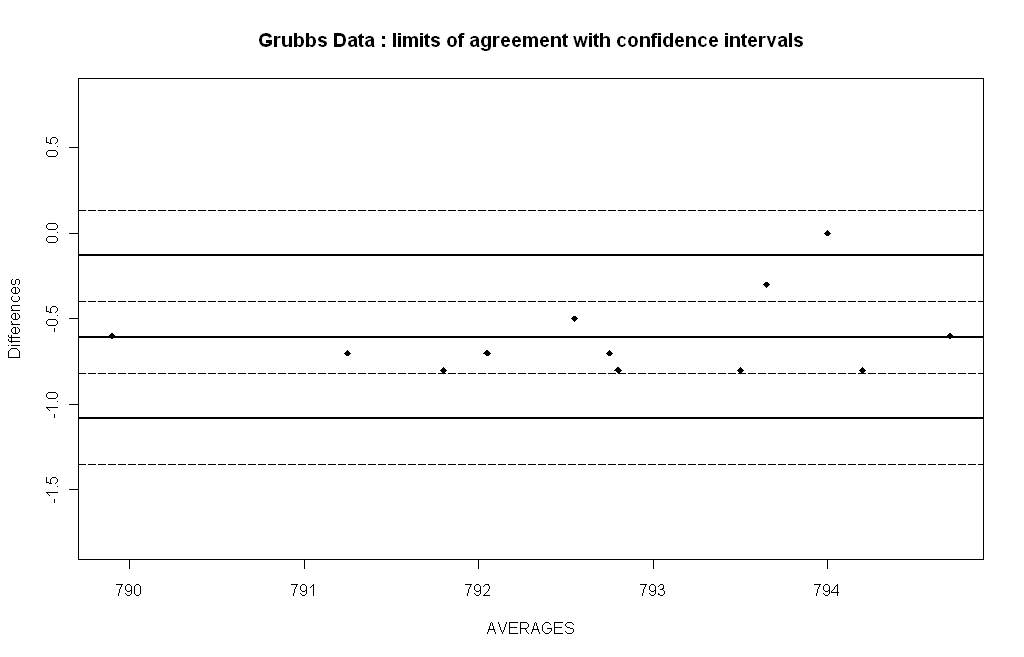
\includegraphics[width=125mm]{images/GrubbsLOAwCIs.jpeg}
%  \caption{Limits of agreement with confidence intervals}\label{LOAwCIs}
%\end{center}
%\end{figure}



















	
	\subsection*{What are Tolerance Intervals?}
	A tolerance interval is a statistical interval within which, with some confidence level, a specified proportion of a population falls.
	The Engineering Statistics Handbook describes the difference: Confidence limits are limits within which we expect a given population parameter, such as the mean, to lie. Statistical tolerance limits are limits within which we expect a stated proportion of the population to lie.
	
	It is useful to make the distinction between tolerance intervals and confidence intervals clear. The confidence interval describes a single-valued population parameter, commonly the mean, with a specified confidence level. The tolerance interval, on the other hand, describes the range of data values that includes a specific proportion of the population.
	
	As discussed in Vardeman (1992), the tolerance interval is not as widely used as the confidence interval and prediction interval, largely because of the emphasis placed on these in undergraduate teaching. Furthermore, Vardeman(1992) argues this lack of awareness can lead to misuse of confidence intervals where other types of intervals are more appropriate.
	Curiously Carstensen et al (2008) describe the Limits of agreement as a prediction interval, although stating that it is formulated in correctly for that purpose.
	
	\subsection*{Why Tolerance Intervals are appropriate?}
	It is clear from the definition of Tolerance intervals that they function precisely as Bland-Altman intend.
	Total Deviation Index and Coverage Probability
	
	The Coverage Probability describes the proportion captured within a pre-specified boundary of the absolute paired-measurement differences from two methods of measurement, i.e., the value of k such that P(|D| <k) = pk.




















\addcontentsline{toc}{section}{Bibliography}
\bibliography{DB-txfrbib}
\end{document}
	